    \section{Algorithms to get a feeling}

    \subsection{Выпуклая оболочка}

    \begin{frame}{Выпуклое множество}
        \vspace{2mm}

        \begin{defn}

            Множество $S$~--- \alert{выпуклое}, если оно вместе с любыми двумя точками содержит отрезок между ними.

        \end{defn}

        \begin{center}

        \begin{tikzpicture}[scale = 0.5]
        \begin{scope}
        \coordinate (a) at (0,0); \coordinate (b) at (-1,2); \coordinate (c) at (1,5); \coordinate (d) at (6,6); \coordinate (e) at (8,2); \coordinate (f) at (4,-1);
        \draw[fill4, fill = fill4] (a) circle (0.07);\draw[fill4, fill = fill4] (b) circle (0.07); \draw[fill4, fill = fill4] (c) circle (0.07); \draw[fill4, fill = fill4] (d) circle (0.07); \draw[fill4, fill = fill4] (e) circle (0.07); \draw[fill4, fill = fill4] (f) circle (0.07);
        \draw[fill4, fill=fill4, fill opacity=0.5, draw opacity = 0] (a)--(b)--(c)--(d)--(e)--(f)--cycle;
        \end{scope}
        \begin{scope}[xshift=12.5cm]
        \coordinate (a) at (0,0); \coordinate (b) at (-1,2); \coordinate (c) at (1,5); \coordinate (d) at (2,1); \coordinate (e) at (8,2); \coordinate (f) at (4, -1); \coordinate (g) at (1, 3); \coordinate (h) at (5, 1);
        \draw[fill4, fill = fill4] (a) circle (0.07);\draw[fill4, fill = fill4] (b) circle (0.07); \draw[fill4, fill = fill4] (c) circle (0.07); \draw[fill4, fill = fill4] (d) circle (0.07); \draw[fill4, fill = fill4] (e) circle (0.07); \draw[fill4, fill = fill4] (f) circle (0.07); \draw[fill1, fill = fill1] (g) circle (0.07); \draw[fill1, fill = fill1] (h) circle (0.07);
        \draw[fill4, fill=fill4, fill opacity=0.5, draw opacity = 0] (a)--(b)--(c)--(d)--(e)--(f)--cycle;
        \draw[fill1, thick] (g)--(h);
        \end{scope}
        \end{tikzpicture}
        \end{center}

    \end{frame}

    \begin{frame}{Выпуклая оболочка}
        
        \vspace{3mm}
        \begin{defn}

            \alert{Выпуклая оболочка $\mathcal{C}\mathcal{H}(S)$} множества $S$~--- наименьшее выпуклое множество, содержащее $S$.

        \end{defn}

        \begin{center}
        \begin{tikzpicture}[scale = 0.4]

        \coordinate (a) at (0,0); \coordinate (b) at (-2,5); \coordinate (c) at (4,10); \coordinate (d) at (12,6); \coordinate (e) at (10,-2);
        \draw[fill4, fill = fill4] (a) circle (0.07);\draw[fill4, fill = fill4] (b) circle (0.07); \draw[fill4, fill = fill4] (c) circle (0.07); \draw[fill4, fill = fill4] (d) circle (0.07); \draw[fill4, fill = fill4] (e) circle (0.07);
        \draw[fill4, fill = fill4] (2, 3) circle (0.07);\draw[fill4, fill = fill4] (4, 7) circle (0.07); \draw[fill4, fill = fill4] (9, 3) circle (0.07); \draw[fill4, fill = fill4] (5, 1) circle (0.07); \draw[fill4, fill = fill4] (6, 3) circle (0.07);
        \draw[fill4, fill=fill4, fill opacity=0.5, draw opacity = 0] (a)--(b)--(c)--(d)--(e)--cycle;

        \end{tikzpicture}
        \end{center}

    \end{frame}

    \begin{frame}{Вычисление выпуклой оболочки}

        \begin{task}
		Дано множество $S \subset \mathbb{R}^2$, $|S| = n$. Требуется найти \\
		координаты вершин его выпуклой оболочки $\mathcal{C}\mathcal{H}(S)$ \\
		в порядке против часовой стрелки.
        \end{task}

    \end{frame}

    \begin{frame}{Вычисление выпуклой оболочки}

        Есть много алгоритмов вычисления выпуклой оболочки на плоскости.
        Большиство из них напоминают алгоритмы сортировок, к примеру

        \begin{itemize}
            \item Алгоритм Джарвиса~--- Selection Sort.
            \item Quick Hull~--- Quick Sort.
            \item Алгоритм <<Разделяй и властвуй>>~--- Merge Sort.
        \end{itemize}

    \end{frame}

    \begin{frame}{Алгоритмы <<Разделяй и властвуй>>}

        Из представленных выше мы рассмотрим алгоритм {\it Divide-and-conquer}. \\

        Все алгоритмы <<Divide-and-Conquer>> имеют одну идею:

        \begin{itemize}

            \item Разбить задачу на подзадачи, от них вызываться рекурсивно.

            \item Научиться быстро сливать подзадачи.

        \end{itemize}

    \end{frame}

    \subsection{Алгоритм $D\&C$ для выпуклой оболочки}

    \begin{frame}{Алгоритм $D\&C$ для $\mathcal{C}\mathcal{H}$: описание}
        \begin{itemize}
            \item $n \le 3 \Rightarrow$ <<brute force>>.
            \item $n \ge 4 \Rightarrow$ разбиваем  $S$ на два примерно равных подмножества по $x$--координате, вызываемся на них рекурсивно.
        \end{itemize}


        \begin{center}
        \begin{tikzpicture}[scale = 0.33]
        % first part:
        \coordinate (a) at (0,0); \coordinate (b) at (-3,4); \coordinate (c) at (-2,7); \coordinate (d) at (2,8); \coordinate (e) at (3,5);
        \draw[fill5, fill = fill5] (a) circle (0.07); \draw[fill5, fill = fill5] (b) circle (0.07); \draw[fill5, fill = fill5] (c) circle (0.07); \draw[fill5, fill = fill5] (d) circle (0.07); \draw[fill5, fill = fill5] (e) circle (0.07);
        \draw[fill5, fill=fill5, fill opacity=0.5, draw opacity = 0] (a)--(b)--(c)--(d)--(e)--cycle;
        % second part:
        \coordinate (f) at (9,0); \coordinate (g) at (5,2); \coordinate (h) at (6,6); \coordinate (k) at (11,7); \coordinate (l) at (13,4);
        \draw[fill5, fill = fill5] (f) circle (0.07); \draw[fill5, fill = fill5] (g) circle (0.07); \draw[fill5, fill = fill5] (h) circle (0.07); \draw[fill5, fill = fill5] (k) circle (0.07); \draw[fill5, fill = fill5] (l) circle (0.07);
        \draw[fill5, fill=fill5, fill opacity=0.5, draw opacity = 0] (f)--(g)--(h)--(k)--(l)--cycle;
        % vertical line
        \draw[fill1, dashed, thick] (4, 10)--(4, -1.5);
        % some random dots inside:
        \draw[fill5, fill = fill5] (-1.95, 6) circle (0.07); \draw[fill5, fill = fill5] (0.05, 5) circle (0.07); \draw[fill5, fill = fill5] (-1, 3) circle (0.07); \draw[fill5, fill = fill5] (1.95, 4) circle (0.07); \draw[fill5, fill = fill5] (1, 7) circle (0.07); \draw[fill5, fill = fill5] (0.1 , 1) circle (0.07);
        \draw[fill5, fill = fill5] (6, 4) circle (0.07); \draw[fill5, fill = fill5] (7, 2) circle (0.07); \draw[fill5, fill = fill5] (8, 5.5) circle (0.07); \draw[fill5, fill = fill5] (10, 6.2) circle (0.07); \draw[fill5, fill = fill5] (12, 5) circle (0.07); \draw[fill5, fill = fill5] (9.2, 1) circle (0.07); \draw[fill5, fill = fill5] (11, 3) circle (0.07); \draw[fill5, fill = fill5] (9.6, 3.5) circle (0.07); \draw[fill5, fill = fill5] (7.5, 3.52) circle (0.07);
        \end{tikzpicture}
        \end{center}

    \end{frame}

    \begin{frame}{Алгоритм $D\&C$ для $\mathcal{C}\mathcal{H}$: слияние подзадач}

        Для слияния подзадач будем считать \alert{верхнюю} и \alert{нижнюю касательные}.

        \begin{center}
        \begin{tikzpicture}[scale = 0.45]
        % first part:
        \coordinate (a) at (0,0); \coordinate (b) at (-3,4); \coordinate (c) at (-2,7); \coordinate (d) at (2,8); \coordinate (e) at (3,5);
        \draw[fill5, fill = fill5] (a) circle (0.07); \draw[fill5, fill = fill5] (b) circle (0.07); \draw[fill5, fill = fill5] (c) circle (0.07); \draw[fill5, fill = fill5] (d) circle (0.07); \draw[fill5, fill = fill5] (e) circle (0.07);
        \draw[fill5, fill=fill5, fill opacity=0.5, draw opacity = 0] (a)--(b)--(c)--(d)--(e)--cycle;
        % second part:
        \coordinate (f) at (9,0); \coordinate (g) at (5,2); \coordinate (h) at (6,6); \coordinate (k) at (11,7); \coordinate (l) at (13,4);
        \draw[fill5, fill = fill5] (f) circle (0.07); \draw[fill5, fill = fill5] (g) circle (0.07); \draw[fill5, fill = fill5] (h) circle (0.07); \draw[fill5, fill = fill5] (k) circle (0.07); \draw[fill5, fill = fill5] (l) circle (0.07);
        \draw[fill5, fill=fill5, fill opacity=0.5, draw opacity = 0] (f)--(g)--(h)--(k)--(l)--cycle;
        % vertical line
        \draw[fill1, dashed, thick] (4, 10)--(4, -1.5);
        % some random dots inside:
        \draw[fill5, fill = fill5] (-1.95, 6) circle (0.07); \draw[fill5, fill = fill5] (0.05, 5) circle (0.07); \draw[fill5, fill = fill5] (-1, 3) circle (0.07); \draw[fill5, fill = fill5] (1.95, 4) circle (0.07); \draw[fill5, fill = fill5] (1, 7) circle (0.07); \draw[fill5, fill = fill5] (0.1 , 1) circle (0.07);
        \draw[fill5, fill = fill5] (6, 4) circle (0.07); \draw[fill5, fill = fill5] (7, 2) circle (0.07); \draw[fill5, fill = fill5] (8, 5.5) circle (0.07); \draw[fill5, fill = fill5] (10, 6.2) circle (0.07); \draw[fill5, fill = fill5] (12, 5) circle (0.07); \draw[fill5, fill = fill5] (9.2, 1) circle (0.07); \draw[fill5, fill = fill5] (11, 3) circle (0.07); \draw[fill5, fill = fill5] (9.6, 3.5) circle (0.07); \draw[fill5, fill = fill5] (7.5, 3.52) circle (0.07);
        % upper tangent
        \draw[fill4, thick] (2, 8)--(11, 7);
        % lower tangent
        \draw[fill4, thick] (0, 0)--(9,0);
        \end{tikzpicture}
        \end{center}

    \end{frame}

    \begin{frame}{Алгоритм $D\&C$ для $\mathcal{C}\mathcal{H}$: верхняя и нижняя касательные}

        Идея вычисления: поднимаем тот конец отрезка,\\ который можем поднять.

        \begin{center}
        \begin{tikzpicture}[scale = 0.45]
        % first part:
        \coordinate (a) at (0,0); \coordinate (b) at (-3,4); \coordinate (c) at (-2,7); \coordinate (d) at (2,8); \coordinate (e) at (3,5);
        \draw[fill5, fill = fill5] (a) circle (0.07); \draw[fill5, fill = fill5] (b) circle (0.07); \draw[fill5, fill = fill5] (c) circle (0.07); \draw[fill5, fill = fill5] (d) circle (0.07); \draw[fill5, fill = fill5] (e) circle (0.07);
        \draw[fill5, fill=fill5, fill opacity=0.5, draw opacity = 0] (a)--(b)--(c)--(d)--(e)--cycle;
        % second part:
        \coordinate (f) at (9,0); \coordinate (g) at (5,2); \coordinate (h) at (6,6); \coordinate (k) at (11,7); \coordinate (l) at (13,4);
        \draw[fill5, fill = fill5] (f) circle (0.07); \draw[fill5, fill = fill5] (g) circle (0.07); \draw[fill5, fill = fill5] (h) circle (0.07); \draw[fill5, fill = fill5] (k) circle (0.07); \draw[fill5, fill = fill5] (l) circle (0.07);
        \draw[fill5, fill=fill5, fill opacity=0.5, draw opacity = 0] (f)--(g)--(h)--(k)--(l)--cycle;
        % vertical line
        \draw[fill1, dashed, thick] (4, 10)--(4, -1.5);
        % some random dots inside:
        \draw[fill5, fill = fill5] (-1.95, 6) circle (0.07); \draw[fill5, fill = fill5] (0.05, 5) circle (0.07); \draw[fill5, fill = fill5] (-1, 3) circle (0.07); \draw[fill5, fill = fill5] (1.95, 4) circle (0.07); \draw[fill5, fill = fill5] (1, 7) circle (0.07); \draw[fill5, fill = fill5] (0.1 , 1) circle (0.07);
        \draw[fill5, fill = fill5] (6, 4) circle (0.07); \draw[fill5, fill = fill5] (7, 2) circle (0.07); \draw[fill5, fill = fill5] (8, 5.5) circle (0.07); \draw[fill5, fill = fill5] (10, 6.2) circle (0.07); \draw[fill5, fill = fill5] (12, 5) circle (0.07); \draw[fill5, fill = fill5] (9.2, 1) circle (0.07); \draw[fill5, fill = fill5] (11, 3) circle (0.07); \draw[fill5, fill = fill5] (9.6, 3.5) circle (0.07); \draw[fill5, fill = fill5] (7.5, 3.52) circle (0.07);
        % upper tangent
        \draw[fill4, dashed, thick] (-3, 4)--(13, 4);
        \draw[fill4, thick] (b) circle (0.3);
        \draw[fill4, thick] (l) circle (0.3);
        \end{tikzpicture}
        \end{center}

    \end{frame}

    \begin{frame}{Алгоритм $D\&C$ для $\mathcal{C}\mathcal{H}$: верхняя и нижняя касательные}

        Идея вычисления: поднимаем тот конец отрезка,\\ который можем поднять.

        \begin{center}
        \begin{tikzpicture}[scale = 0.45]
        % first part:
        \coordinate (a) at (0,0); \coordinate (b) at (-3,4); \coordinate (c) at (-2,7); \coordinate (d) at (2,8); \coordinate (e) at (3,5);
        \draw[fill5, fill = fill5] (a) circle (0.07); \draw[fill5, fill = fill5] (b) circle (0.07); \draw[fill5, fill = fill5] (c) circle (0.07); \draw[fill5, fill = fill5] (d) circle (0.07); \draw[fill5, fill = fill5] (e) circle (0.07);
        \draw[fill5, fill=fill5, fill opacity=0.5, draw opacity = 0] (a)--(b)--(c)--(d)--(e)--cycle;
        % second part:
        \coordinate (f) at (9,0); \coordinate (g) at (5,2); \coordinate (h) at (6,6); \coordinate (k) at (11,7); \coordinate (l) at (13,4);
        \draw[fill5, fill = fill5] (f) circle (0.07); \draw[fill5, fill = fill5] (g) circle (0.07); \draw[fill5, fill = fill5] (h) circle (0.07); \draw[fill5, fill = fill5] (k) circle (0.07); \draw[fill5, fill = fill5] (l) circle (0.07);
        \draw[fill5, fill=fill5, fill opacity=0.5, draw opacity = 0] (f)--(g)--(h)--(k)--(l)--cycle;
        % vertical line
        \draw[fill1, dashed, thick] (4, 10)--(4, -1.5);
        % some random dots inside:
        \draw[fill5, fill = fill5] (-1.95, 6) circle (0.07); \draw[fill5, fill = fill5] (0.05, 5) circle (0.07); \draw[fill5, fill = fill5] (-1, 3) circle (0.07); \draw[fill5, fill = fill5] (1.95, 4) circle (0.07); \draw[fill5, fill = fill5] (1, 7) circle (0.07); \draw[fill5, fill = fill5] (0.1 , 1) circle (0.07);
        \draw[fill5, fill = fill5] (6, 4) circle (0.07); \draw[fill5, fill = fill5] (7, 2) circle (0.07); \draw[fill5, fill = fill5] (8, 5.5) circle (0.07); \draw[fill5, fill = fill5] (10, 6.2) circle (0.07); \draw[fill5, fill = fill5] (12, 5) circle (0.07); \draw[fill5, fill = fill5] (9.2, 1) circle (0.07); \draw[fill5, fill = fill5] (11, 3) circle (0.07); \draw[fill5, fill = fill5] (9.6, 3.5) circle (0.07); \draw[fill5, fill = fill5] (7.5, 3.52) circle (0.07);
        % upper tangent
        \draw[fill4, dashed, thick] (-2, 7)--(13, 4);
        \draw[fill4, dashed, thick] (-3, 4)--(13, 4);
        \draw[->, fill4, dashed, thick] (-3, 4)--(-2, 7);
        \draw[fill4,  thick] (b) circle (0.3);
        \draw[fill4,  thick] (l) circle (0.3);
        \end{tikzpicture}
        \end{center}

    \end{frame}

    \begin{frame}{Алгоритм $D\&C$ для $\mathcal{C}\mathcal{H}$: верхняя и нижняя касательные}

        Идея вычисления: поднимаем тот конец отрезка,\\ который можем поднять.

        \begin{center}
        \begin{tikzpicture}[scale = 0.45]
        % first part:
        \coordinate (a) at (0,0); \coordinate (b) at (-3,4); \coordinate (c) at (-2,7); \coordinate (d) at (2,8); \coordinate (e) at (3,5);
        \draw[fill5, fill = fill5] (a) circle (0.07); \draw[fill5, fill = fill5] (b) circle (0.07); \draw[fill5, fill = fill5] (c) circle (0.07); \draw[fill5, fill = fill5] (d) circle (0.07); \draw[fill5, fill = fill5] (e) circle (0.07);
        \draw[fill5, fill=fill5, fill opacity=0.5, draw opacity = 0] (a)--(b)--(c)--(d)--(e)--cycle;
        % second part:
        \coordinate (f) at (9,0); \coordinate (g) at (5,2); \coordinate (h) at (6,6); \coordinate (k) at (11,7); \coordinate (l) at (13,4);
        \draw[fill5, fill = fill5] (f) circle (0.07); \draw[fill5, fill = fill5] (g) circle (0.07); \draw[fill5, fill = fill5] (h) circle (0.07); \draw[fill5, fill = fill5] (k) circle (0.07); \draw[fill5, fill = fill5] (l) circle (0.07);
        \draw[fill5, fill=fill5, fill opacity=0.5, draw opacity = 0] (f)--(g)--(h)--(k)--(l)--cycle;
        % vertical line
        \draw[fill1, dashed, thick] (4, 10)--(4, -1.5);
        % some random dots inside:
        \draw[fill5, fill = fill5] (-1.95, 6) circle (0.07); \draw[fill5, fill = fill5] (0.05, 5) circle (0.07); \draw[fill5, fill = fill5] (-1, 3) circle (0.07); \draw[fill5, fill = fill5] (1.95, 4) circle (0.07); \draw[fill5, fill = fill5] (1, 7) circle (0.07); \draw[fill5, fill = fill5] (0.1 , 1) circle (0.07);
        \draw[fill5, fill = fill5] (6, 4) circle (0.07); \draw[fill5, fill = fill5] (7, 2) circle (0.07); \draw[fill5, fill = fill5] (8, 5.5) circle (0.07); \draw[fill5, fill = fill5] (10, 6.2) circle (0.07); \draw[fill5, fill = fill5] (12, 5) circle (0.07); \draw[fill5, fill = fill5] (9.2, 1) circle (0.07); \draw[fill5, fill = fill5] (11, 3) circle (0.07); \draw[fill5, fill = fill5] (9.6, 3.5) circle (0.07); \draw[fill5, fill = fill5] (7.5, 3.52) circle (0.07);
        % upper tangent
        \draw[fill4, dashed, thick] (-2, 7)--(13, 4);
        \draw[fill4, dashed, thick] (2, 8)--(13, 4);
        \draw[->, fill4, dashed, thick] (-2, 7)--(2, 8);
        \draw[fill4,  thick] (c) circle (0.3);
        \draw[fill4,  thick] (l) circle (0.3);
        \end{tikzpicture}
        \end{center}

    \end{frame}

    \begin{frame}{Алгоритм $D\&C$ для $\mathcal{C}\mathcal{H}$: верхняя и нижняя касательные}

        Идея вычисления: поднимаем тот конец отрезка,\\ который можем поднять.

        \begin{center}
        \begin{tikzpicture}[scale = 0.45]
        % first part:
        \coordinate (a) at (0,0); \coordinate (b) at (-3,4); \coordinate (c) at (-2,7); \coordinate (d) at (2,8); \coordinate (e) at (3,5);
        \draw[fill5, fill = fill5] (a) circle (0.07); \draw[fill5, fill = fill5] (b) circle (0.07); \draw[fill5, fill = fill5] (c) circle (0.07); \draw[fill5, fill = fill5] (d) circle (0.07); \draw[fill5, fill = fill5] (e) circle (0.07);
        \draw[fill5, fill=fill5, fill opacity=0.5, draw opacity = 0] (a)--(b)--(c)--(d)--(e)--cycle;
        % second part:
        \coordinate (f) at (9,0); \coordinate (g) at (5,2); \coordinate (h) at (6,6); \coordinate (k) at (11,7); \coordinate (l) at (13,4);
        \draw[fill5, fill = fill5] (f) circle (0.07); \draw[fill5, fill = fill5] (g) circle (0.07); \draw[fill5, fill = fill5] (h) circle (0.07); \draw[fill5, fill = fill5] (k) circle (0.07); \draw[fill5, fill = fill5] (l) circle (0.07);
        \draw[fill5, fill=fill5, fill opacity=0.5, draw opacity = 0] (f)--(g)--(h)--(k)--(l)--cycle;
        % vertical line
        \draw[fill1, dashed, thick] (4, 10)--(4, -1.5);
        % some random dots inside:
        \draw[fill5, fill = fill5] (-1.95, 6) circle (0.07); \draw[fill5, fill = fill5] (0.05, 5) circle (0.07); \draw[fill5, fill = fill5] (-1, 3) circle (0.07); \draw[fill5, fill = fill5] (1.95, 4) circle (0.07); \draw[fill5, fill = fill5] (1, 7) circle (0.07); \draw[fill5, fill = fill5] (0.1 , 1) circle (0.07);
        \draw[fill5, fill = fill5] (6, 4) circle (0.07); \draw[fill5, fill = fill5] (7, 2) circle (0.07); \draw[fill5, fill = fill5] (8, 5.5) circle (0.07); \draw[fill5, fill = fill5] (10, 6.2) circle (0.07); \draw[fill5, fill = fill5] (12, 5) circle (0.07); \draw[fill5, fill = fill5] (9.2, 1) circle (0.07); \draw[fill5, fill = fill5] (11, 3) circle (0.07); \draw[fill5, fill = fill5] (9.6, 3.5) circle (0.07); \draw[fill5, fill = fill5] (7.5, 3.52) circle (0.07);
        % upper tangent
        \draw[fill4, dashed, thick] (2, 8)--(13, 4);
        \draw[->, fill4, dashed, thick] (l)--(k);
        \draw[fill4, thick] (d)--(k);
        \draw[fill4,  thick] (d) circle (0.3);
        \draw[fill4,  thick] (l) circle (0.3);
        \end{tikzpicture}
        \end{center}

    \end{frame}

    \begin{frame}{Алгоритм $D\&C$ для $\mathcal{C}\mathcal{H}$: оценка времени работы}

        Количество точек в подзадаче сокращается хотя бы в два раза, на слияние мы тратим линейное время
        \[ T(n) = 2T\bigg(\frac{n}{2}\bigg) + O(n) \]
        \begin{center}
        \tikz
        \node {$T(n)$}[sibling distance = 2.5cm]
        child { node {$T(\frac{n}{2})$} child{node{$T(\frac{n}{4})$}} child {node[xshift = -1cm]{$T(\frac{n}{4})$}}}
        child { node {$T(\frac{n}{2})$} child{node[xshift = 1cm]{$T(\frac{n}{4})$}} child{node{$T(\frac{n}{4})$}}};
        \end{center}

    \end{frame}

    \begin{frame}{Алгоритм $D\&C$ для $\mathcal{C}\mathcal{H}$: оценка времени работы}
        \[ T(n) = 2T\bigg(\frac{n}{2}\bigg) + O(n) \]

        Распишем это:

        \[ T(n) =
      O \lr*{
         n \cdot \lr*{
            \frac{2}{2} + \lr*{
               \frac{2}{2}
            }^2 + \ldots + \lr*{
               \frac{2}{2}
            }^{\log_{2}(n)}
         }
      } = O \lr*{
         n \cdot \sum\limits_{k = 1}^{\log_2{n}} 1
      } = O \lr*{n\log_2\lr*{n}}.\]

    \end{frame}

    \subsection{Касательная к выпуклому многоугольнику}

    \begin{frame}{Касательная к выпуклому многоугольнику}

        \begin{task}
            Дан выпуклый многоугольник $\mathcal{P} \subset \mathbb{R}^2$ и точка $X_0(x_0, y_0) \in \mathbb{R}^2$.
            Найти касательную к $\mathcal{P}$ из точки $X_0(x_0, y_0)$.
        \end{task}

    \end{frame}

    \begin{frame}{Касательная к выпуклому многоугольнику: алгоритм}

        Каждой вершине сопоставим \emph{аргумент}~--- угол, под которым она видна их точки $X_0$.

        \begin{center}
        \begin{tikzpicture}[scale = 0.45]
        % polygone:
        \coordinate (a) at (0,0); \coordinate (b) at (-2,4); \coordinate (c) at (0,7); \coordinate (d) at (3,8); \coordinate (e) at (7,6); \coordinate (f) at (8, 1); \coordinate (g) at (4, -1); \coordinate[label= below :$X_0$] (p) at (-5, 1); \coordinate (l) at (-1, 1);
        \draw[fill5, fill = fill5] (a) circle (0.13); \draw[fill5, fill = fill5] (b) circle (0.13); \draw[fill5, fill = fill5] (c) circle (0.13); \draw[fill5, fill = fill5] (d) circle (0.13); \draw[fill5, fill = fill5] (e) circle (0.13); \draw[fill5, fill = fill5] (f) circle (0.13); \draw[fill5, fill = fill5] (g) circle (0.13);
        \draw[fill5, fill=fill5, fill opacity=0.5, draw opacity = 0] (a)--(b)--(c)--(d)--(e)--(f)--(g)--cycle;
        % point:
        \draw[fill5, fill = fill5] (p) circle (0.13);
        \draw[fill4, -> , thick] (-10, 1)--(13, 1);
        \draw[fill4, thick] (-5, 1)--(2, 8);
        \draw pic[draw, <-,  thick, fill1, angle radius=1cm, shift={(6mm,1mm)}] {angle=l--p--b};
        \end{tikzpicture}
        \end{center}

    \end{frame}

    \begin{frame}{Касательная к выпуклому многоугольнику: алгоритм}

        У нужной вершины $v_i$ аргументы будут расположены так:

        \begin{center}
        \begin{tikzpicture}[scale = 0.3]
        % polygone:
        \coordinate[fill4, label=right:$v_{i - 1}$] (a) at (0,0); \coordinate[fill4, label=left:$v_i$] (b) at (-2,3); \coordinate[fill4, label=right:$v_{i + 1}$] (c) at (1, 6);
        \draw[fill4, fill = fill4] (a) circle (0.13); \draw[fill4, fill = fill4] (b) circle (0.13); \draw[fill4, fill = fill4] (c) circle (0.13);
        \draw[fill4, thick] (a)--(b) node[xshift = 0.1cm, yshift= -0.7cm]{$\vee$};
        \draw[fill4, thick] (b)--(c) node[xshift = -0.6cm, yshift = -0.25cm]{$\wedge$};
        \end{tikzpicture}
        \end{center}

        Как понять, с какой стороны нужная вершина:

        \begin{center}
        \begin{tikzpicture}[scale = 0.3]
        \begin{scope}
        % first:
        \coordinate[fill4, label=right:$v_{i - 1}$] (a) at (0,0); \coordinate[fill4, label=left:$v_i$] (b) at (-2,3); \coordinate[fill4, label=right:$v_{i + 1}$] (c) at (1, 6);
        \draw[fill4, fill = fill4] (a) circle (0.13); \draw[fill4, fill = fill4] (b) circle (0.13); \draw[fill4, fill = fill4] (c) circle (0.13);
        \draw[fill4, thick, <-] (a)--(b) node[xshift = 0.1cm, yshift= -0.7cm]{$\wedge$};
        \draw[fill4, thick, <-] (b)--(c) node[xshift = -0.6cm, yshift = -0.25cm]{$\wedge$};
        \end{scope}
        \begin{scope}[xshift = 10cm]
        % second:
        \coordinate[fill4, label=right:$v_{i - 1}$] (a) at (0,0); \coordinate[fill4, label=left:$v_i$] (b) at (-2,3); \coordinate[fill4, label=right:$v_{i + 1}$] (c) at (1, 6);
        \draw[fill4, fill = fill4] (a) circle (0.13); \draw[fill4, fill = fill4] (b) circle (0.13); \draw[fill4, fill = fill4] (c) circle (0.13);
        \draw[fill4, thick, ->] (a)--(b) node[xshift = 0.1cm, yshift= -0.7cm]{$\vee$};
        \draw[fill4, thick, ->] (b)--(c) node[xshift = -0.6cm, yshift = -0.25cm]{$\vee$};
        \end{scope}
        \end{tikzpicture}

        \end{center}
    \end{frame}

     \begin{frame}{Касательная к выпуклому многоугольнику: алгоритм}
         \begin{itemize}

             \item Выберем две вершины на противоположных сторонах~--- $v_0$ и $v_{\frac{n}{2}}$,
                   посчитаем аргументы их и их соседей.

             \item Получим один из случаев:

         \end{itemize}
            \begin{center}
            \begin{tikzpicture}[scale = 0.3]
            \begin{scope}
            % first:
            \node at (-2, 7) {1};
            \draw[thick] (-2, 7)  circle (0.7);
            \coordinate[fill4, label=right:$v_{n}$] (a) at (0,0); \coordinate[fill4, label=left:$v_0$] (b) at (-2,3); \coordinate[fill4, label=right:$v_{1}$] (c) at (1, 6);
            \draw[fill4, fill = fill4] (a) circle (0.13); \draw[fill4, fill = fill4] (b) circle (0.13); \draw[fill4, fill = fill4] (c) circle (0.13);
            \draw[fill4, thick, ->] (a)--(b) node[xshift = 0.1cm, yshift= -0.7cm]{$\vee$};
            \draw[fill4, thick, ->] (b)--(c) node[xshift = -0.6cm, yshift = -0.25cm]{$\vee$};
            \end{scope}

            \begin{scope}[xshift = 10cm]
            % second:
            \coordinate[fill4, label=right:$v_{\frac{n}{2} - 1}$] (a) at (0,0); \coordinate[fill4, label=left:$v_{\frac{n}{2}}$] (b) at (-2,3); \coordinate[fill4, label=right:$v_{\frac{n}{2} + 1}$] (c) at (1, 6);
            \draw[fill4, fill = fill4] (a) circle (0.13); \draw[fill4, fill = fill4] (b) circle (0.13); \draw[fill4, fill = fill4] (c) circle (0.13);
            \draw[fill4, thick, ->] (a)--(b) node[xshift = 0.1cm, yshift= -0.7cm]{$\vee$};
            \draw[fill4, thick, ->] (b)--(c) node[xshift = -0.6cm, yshift = -0.25cm]{$\vee$};
            \end{scope}

            \begin{scope}[xshift = 20cm]
            % third:
            \node at (-2, 7) {2};
            \draw[thick] (-2, 7)  circle (0.7);
            \coordinate[fill4, label=right:$v_{1}$] (a) at (0,0); \coordinate[fill4, label=right:$v_{0}$] (b) at (2,3); \coordinate[fill4, label=right:$v_{n}$] (c) at (-1, 6);
            \draw[fill4, fill = fill4] (a) circle (0.13); \draw[fill4, fill = fill4] (b) circle (0.13); \draw[fill4, fill = fill4] (c) circle (0.13);
            \draw[fill4, thick, <-] (a)--(b) node[xshift = 0.05cm, yshift= -0.42cm]{$\vee$};
            \draw[fill4, thick, <-] (b)--(c) node[xshift = 0.72cm, yshift = -0.4cm]{$\vee$};
            \end{scope}

            \begin{scope}[xshift = 30cm]
            % fourth:
            \coordinate[fill4, label=right:$v_{\frac{n}{2} + 1}$] (a) at (0,0); \coordinate[fill4, label=right:$v_{\frac{n}{2}}$] (b) at (2,3); \coordinate[fill4, label=right:$v_{\frac{n}{2} - 1}$] (c) at (-1, 6);
            \draw[fill4, fill = fill4] (a) circle (0.13); \draw[fill4, fill = fill4] (b) circle (0.13); \draw[fill4, fill = fill4] (c) circle (0.13);
            \draw[fill4, thick, <-] (a)--(b) node[xshift = 0.05cm, yshift= -0.42cm]{$\vee$};
            \draw[fill4, thick, <-] (b)--(c) node[xshift = 0.72cm, yshift = -0.4cm]{$\vee$};
            \end{scope}
            \end{tikzpicture}
            \end{center}

     \end{frame}

    \begin{frame}{Касательная к выпуклому многоугольнику: алгоритм}

        \begin{center}
        \begin{tikzpicture}[scale = 0.3]
        \begin{scope}
        % first:
        \node at (-2, 7) {3};
        \draw[thick] (-2, 7)  circle (0.7);
        \coordinate[fill4, label=right:$v_{n}$] (a) at (0,0); \coordinate[fill4, label=left:$v_0$] (b) at (-2,3); \coordinate[fill4, label=right:$v_{1}$] (c) at (1, 6);
        \draw[fill4, fill = fill4] (a) circle (0.13); \draw[fill4, fill = fill4] (b) circle (0.13); \draw[fill4, fill = fill4] (c) circle (0.13);
        \draw[fill4, thick, ->] (a)--(b) node[xshift = 0.1cm, yshift= -0.7cm]{$\vee$};
        \draw[fill4, thick, ->] (b)--(c) node[xshift = -0.6cm, yshift = -0.27cm]{$\vee$};
        \end{scope}

        \begin{scope}[xshift = 10cm]
        % fourth:
        \coordinate[fill4, label=right:$v_{\frac{n}{2} + 1}$] (a) at (0,0); \coordinate[fill4, label=right:$v_{\frac{n}{2}}$] (b) at (2,3); \coordinate[fill4, label=right:$v_{\frac{n}{2} - 1}$] (c) at (-1, 6);
        \draw[fill4, fill = fill4] (a) circle (0.13); \draw[fill4, fill = fill4] (b) circle (0.13); \draw[fill4, fill = fill4] (c) circle (0.13);
        \draw[fill4, thick, <-] (a)--(b) node[xshift = 0.05cm, yshift= -0.42cm]{$\vee$};
        \draw[fill4, thick, <-] (b)--(c) node[xshift = 0.72cm, yshift = -0.4cm]{$\vee$};
        \end{scope}
        \end{tikzpicture}
        \end{center}

        \begin{itemize}

            \item Каждый раз отбрасываем половину вершин.

            \item После отбрасывания половины добавляем вершину посередине нового промежутка и продолжаем.
        \end{itemize}

    \end{frame}

    \begin{frame}{Кас. к вып. многоуг.: время работы}

        Каждый следующий запрос~--- $O(1)$ проверок ориентации.
        Всего запросов~--- $O(\log(n))$, а значит, время работы~--- $O(\log(n))$.
        
        \vspace{5mm}
        
        \begin{block}{Упражнение.}

            Придумайте алгоритм выпуклой оболочки, использующий алгоритм построения касательной и алгоритм
            $D\&C$. Время работы алгоритма должно составлять $O(n\log(h))$, где $h$~--- количество вершин  в выпуклой оболочке.

        \end{block}

    \end{frame}

    \section{Триангуляция и картинная галерея}

    \begin{frame}{Лемма о триангуляции}

    \vspace{2mm}
    \begin{lm}[О триангуляции]\hypertarget{trianglemm}{}

        Всякий многоугольник можно диагоналями разбить на треугольники, причем полученный граф красится в 3 цвета.

    \end{lm}

    \begin{proof}\let\qed\relax
        Индукция по числу вершин.\\

        \textbf{База:} $n = 3$.\\
        \textbf{Переход:} Находим вершину с  углом $<180^{\circ}$.\\

        \begin{itemize}

            \item Отрезок между соседними  вершинами лежит в многоугольнике:\\
            Отрезаем вершину, красим по индукции, возвращаем, красим в свободный цвет.

        \end{itemize}

    \end{proof}

    \end{frame}

    \begin{frame}{Лемма о триангуляции: доказательство}

    \vspace{2mm}

    \begin{proof}\let\qed\relax

        \begin{center}
        \begin{tikzpicture}[scale = 0.25]
        \begin{scope}
        \coordinate (a) at (0,0); \coordinate (b) at (-3,1); \coordinate (c) at (-2, 5); \coordinate (d) at (1, 7); \coordinate (e) at (4, 4); \coordinate (f) at (7, 6); \coordinate (g) at (8, 1);
        \draw[fill1, fill = fill1] (a) circle (0.1);\draw[fill4, fill = fill4] (b) circle (0.1); \draw[fill4, fill = fill4] (c) circle (0.1); \draw[fill4, fill = fill4] (d) circle (0.1); \draw[fill4, fill = fill4] (e) circle (0.1); \draw[fill4, fill = fill4] (f) circle (0.1); \draw[fill4, fill = fill4] (g) circle (0.1);
        \draw[fill4, thick] (c)--(d)--(e)--(f)--(g)--(a);
        \draw pic[draw, thick, fill1, angle radius=0.2cm, shift={(6mm,1mm)}] {angle=a--b--c};
        \draw[fill1, thick, dashed] (b)--(c);
        \draw[fill1, thick, dashed] (a)--(b);
        \draw[fill1, thick, dashed] (a)--(c);
        \end{scope}
        \begin{scope}[xshift = 15cm]
        \coordinate (a) at (0,0); \coordinate (b) at (-3,1); \coordinate (c) at (-2, 5); \coordinate (d) at (1, 7); \coordinate (e) at (4, 4); \coordinate (f) at (7, 6); \coordinate (g) at (8, 1);
        \draw[fill4, fill = fill4] (a) circle (0.1);\draw[fill4, fill = fill4] (b) circle (0.1); \draw[fill4, fill = fill4] (c) circle (0.1); \draw[fill4, fill = fill4] (d) circle (0.1); \draw[fill4, fill = fill4] (e) circle (0.1); \draw[fill4, fill = fill4] (f) circle (0.1); \draw[fill4, fill = fill4] (g) circle (0.1);
        \draw[fill4, thick] (a)--(c)--(d)--(e)--(f)--(g)--cycle;
        \draw pic[draw,  thick, fill1, angle radius=0.2cm, shift={(6mm,1mm)}] {angle=a--b--c};
        \draw[fill4, thick] (a)--(d);
        \draw[fill4, thick] (a)--(e);
        \draw[fill4, thick] (e)--(g);
        \draw[fill1, dashed, thick] (b)--(c);
        \draw[fill1, dashed, thick] (a)--(b);
        \end{scope}
        \end{tikzpicture}
        \end{center} \vspace{-7mm}

        \begin{itemize}
        \item Отрезок между соседними  вершинами не лежит в многоугольнике:

        \begin{center}
        \begin{tikzpicture}[scale = 0.25]
        \begin{scope}
        \coordinate (a) at (0,0); \coordinate (b) at (3,6); \coordinate (c) at (8, 7); \coordinate (d) at (3, 2); \coordinate (e) at (9, 0); \coordinate (f) at (-2, 7); \coordinate (g) at (7, -2);
        \draw[fill1, fill = fill1] (a) circle (0.1);\draw[fill4, fill = fill4] (b) circle (0.1); \draw[fill4, fill = fill4] (c) circle (0.1); \draw[fill4, fill = fill4] (d) circle (0.1); \draw[fill4, fill = fill4] (e) circle (0.1);
        \draw[fill4, thick] (a)--(b)--(c)--(d)--(e)--cycle;
        \draw[fill1, thick] (b)--(e);
        \draw[fill1, thick] (f)--(g);
        \draw pic[draw,  thick, fill1, angle radius=0.35cm, shift={(6mm,1mm)}] {angle=e--a--b};
        \end{scope}
        \begin{scope}[xshift = 15cm]
        \coordinate (a) at (0,0); \coordinate (b) at (3,7); \coordinate (c) at (8, 7); \coordinate (d) at (3, 2); \coordinate (e) at (11, 0); \coordinate (f) at (-3, 7);
        \draw[fill1, fill = fill1] (a) circle (0.1);\draw[fill4, fill = fill4] (b) circle (0.1); \draw[fill4, fill = fill4] (c) circle (0.1); \draw[fill4, fill = fill4] (d) circle (0.1); \draw[fill4, fill = fill4] (e) circle (0.1);
        \draw[fill4, thick] (a)--(b)--(c)--(d)--(e)--cycle;
        \draw[fill1, thick] (a)--(d);
        \draw[fill4, thick] (b)--(d);
        \draw[fill4, thick] (b)--(d);
        \end{scope}
        \end{tikzpicture}
        \end{center}

    \end{itemize}

    \end{proof}

    \end{frame}

    \subsection{Задача о картинной галерее}

    \begin{frame}{Задача о картинной галерее}

        \begin{task}

            Дана картинная галерея, план которой~--- многоугольник без самопересечений. Какое минимальное число охранников нужно поставить в точках галереи, чтоб
            они просматривали каждую точку?

        \end{task}

    \end{frame}

    \begin{frame}{Задача о картинной галерее: иллюстрация}
\begin{center}
  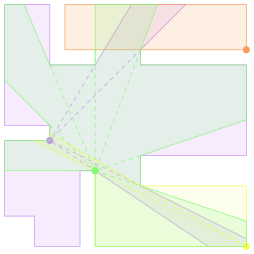
\includegraphics[height=0.84\textheight]{svg/pictGallery}
\end{center}
    \end{frame}

    \begin{frame}{Задача о картинной галерее}
        
        \vspace{2mm}
        \begin{thm}[Хватал]
		Для произвольного $n$-угольника
		достаточно $\lfloor \frac{n}{3} \rfloor$ охранников,\\
		поставленных во внутренних точках, чтобы охранникам\\
		были видны все внутренние точки $n$-угольника.
        \end{thm}

        \begin{block}{Доказательство}
		По \hyperlink{trianglemm}{лемме} строим разбиение
		галереи на треугольники,\\
		вершины раскрашиваются в три цвета. Из этих цветов\\
		выбираем тот, который встречается \emph{не чаще других}.\\
		Ставим охранников в вершины, окрашенные этим цветом.
        \end{block}
    \end{frame}
